\documentclass[14pt]{extarticle}
\usepackage{cmap}
\usepackage[T2A]{fontenc}
\usepackage[utf8]{inputenc}
\usepackage[russian]{babel}
\usepackage[a4paper, left=25mm, right=15mm, top=20mm, bottom=20mm]{geometry}
\usepackage{amsmath, amssymb}
\usepackage{graphicx}
\usepackage{float}
\usepackage{booktabs}
\usepackage{array}
\usepackage{caption}
\usepackage{indentfirst}
\usepackage{enumitem}
\usepackage[hidelinks]{hyperref}
\usepackage{setspace}

\graphicspath{{figures/}}
\captionsetup{labelsep=period, font=small}
\captionsetup[table]{justification=raggedleft, singlelinecheck=false}
\setlength{\parindent}{1.25cm}
\onehalfspacing
\setlist{nosep, leftmargin=1.5cm}
\renewcommand{\arraystretch}{1.12}
\newcommand{\nm}[1]{\overline{#1}}

% ---------- титульный лист ----------
% #1 -- номер работы, #2 -- тема
\newcommand{\itmotitle}[2]{%
\begin{titlepage}
\begin{center}
\singlespacing
Министерство науки и высшего образования Российской Федерации\\[2mm]
Федеральное государственное автономное образовательное учреждение высшего образования
«Национальный исследовательский университет ИТМО»\\
(университет ИТМО)\\[6mm]
Факультет «Систем управления и робототехники»

\vspace{38mm}

{\large\bfseries ОТЧЕТ\\[1mm] О ЛАБОРАТОРНОЙ РАБОТЕ №#1}\\[4mm]
По дисциплине «Электроника и схемотехника»\\[3mm]
на тему:\\[1mm]
{\bfseries «#2»}\\[6mm]
Вариант 2
\end{center}

\vspace{30mm}

\begin{flushright}
\begin{minipage}{0.62\textwidth}
\singlespacing
Преподаватель: Зарина Ольга Андреевна\\[4mm]
Выполнили:\\
Басиони Адельсалам Али Абдельсалам -- 465144\\
Боврджи Тамим Махер Мохаммед -- 412894\\[4mm]
Поток: ЭЛЕК И СХЕМ R БАК 1.2
\end{minipage}
\end{flushright}

\vfill
\begin{center}
г. Санкт-Петербург\\
2026
\end{center}
\end{titlepage}
\setcounter{page}{2}
}


\begin{document}
\itmotitle{7.2}{Последовательные логические элементы: триггеры, регистры, счётчики}

\tableofcontents
\newpage

\section*{Цель работы}
\addcontentsline{toc}{section}{Цель работы}
\begin{itemize}
\item Исследовать работу логических устройств с памятью -- триггеров, регистров и счётчиков.
\item Научиться реализовывать простейшие последовательные схемы, отслеживать состояние и
анализировать переходы между логическими уровнями при подаче тактовых и управляющих сигналов.
\end{itemize}

\section*{Исходные данные}
\addcontentsline{toc}{section}{Исходные данные}
\begin{table}[H]
\caption{Задание по варианту 2}\label{tab:var}
\centering
\small\begin{tabular}{cccc}
\toprule
№ & Тип триггера & Тип регистра & Тип счётчика\\
\midrule
2 & Синхронный RS на И-НЕ & Сдвигающий влево & Синхронный нисходящий\\
\bottomrule
\end{tabular}
\end{table}

\textbf{Условия моделирования.} Схемы собраны в LTspice из стандартных элементов библиотеки
\texttt{Digital}: элементов И (\texttt{and}, выход с инверсией используется как И-НЕ),
\texttt{xor} и D-триггеров \texttt{dflop}, тактируемых передним фронтом. Для всех элементов
задано \texttt{Vhigh=5 Vlow=0 Ref=2.5 Td=10n} (уровни 0/5~В, порог 2,5~В, задержка 10~нс).
Неиспользуемые входы и входы асинхронной установки PRE соединены с общим проводом и
неактивны. Тактовый сигнал -- источник \texttt{PULSE} 0--5~В с периодом 1~мкс;
установочные и информационные сигналы -- источники \texttt{PWL} и \texttt{PULSE}.

% =====================================================================
\section{Синхронный RS-триггер на элементах И-НЕ}
\subsection{Принцип работы и схема}
Триггер состоит из входной (управляющей) ступени -- элементов DD1, DD2 (на схеме A1, A2) --
и асинхронного RS-триггера на элементах A3, A4 с инверсными входами:
\begin{equation}
S' = \overline{S\cdot C},\quad R' = \overline{R\cdot C},\quad
Q=\overline{S'\cdot\nm{Q}},\quad \nm{Q}=\overline{R'\cdot Q}.
\end{equation}
При $C=0$ оба сигнала $S'$ и $R'$ равны 1 и триггер хранит состояние. При $C=1$ сигналы
$S$, $R$ (активный уровень -- 1) проходят на защёлку: $S=1$ устанавливает $Q=1$, $R=1$
сбрасывает $Q=0$, $S=R=0$ -- хранение, $S=R=1$ -- запрещённая комбинация.
Таким образом, триггер управляется уровнем (а не фронтом) сигнала $C$.

\begin{figure}[H]
\centering
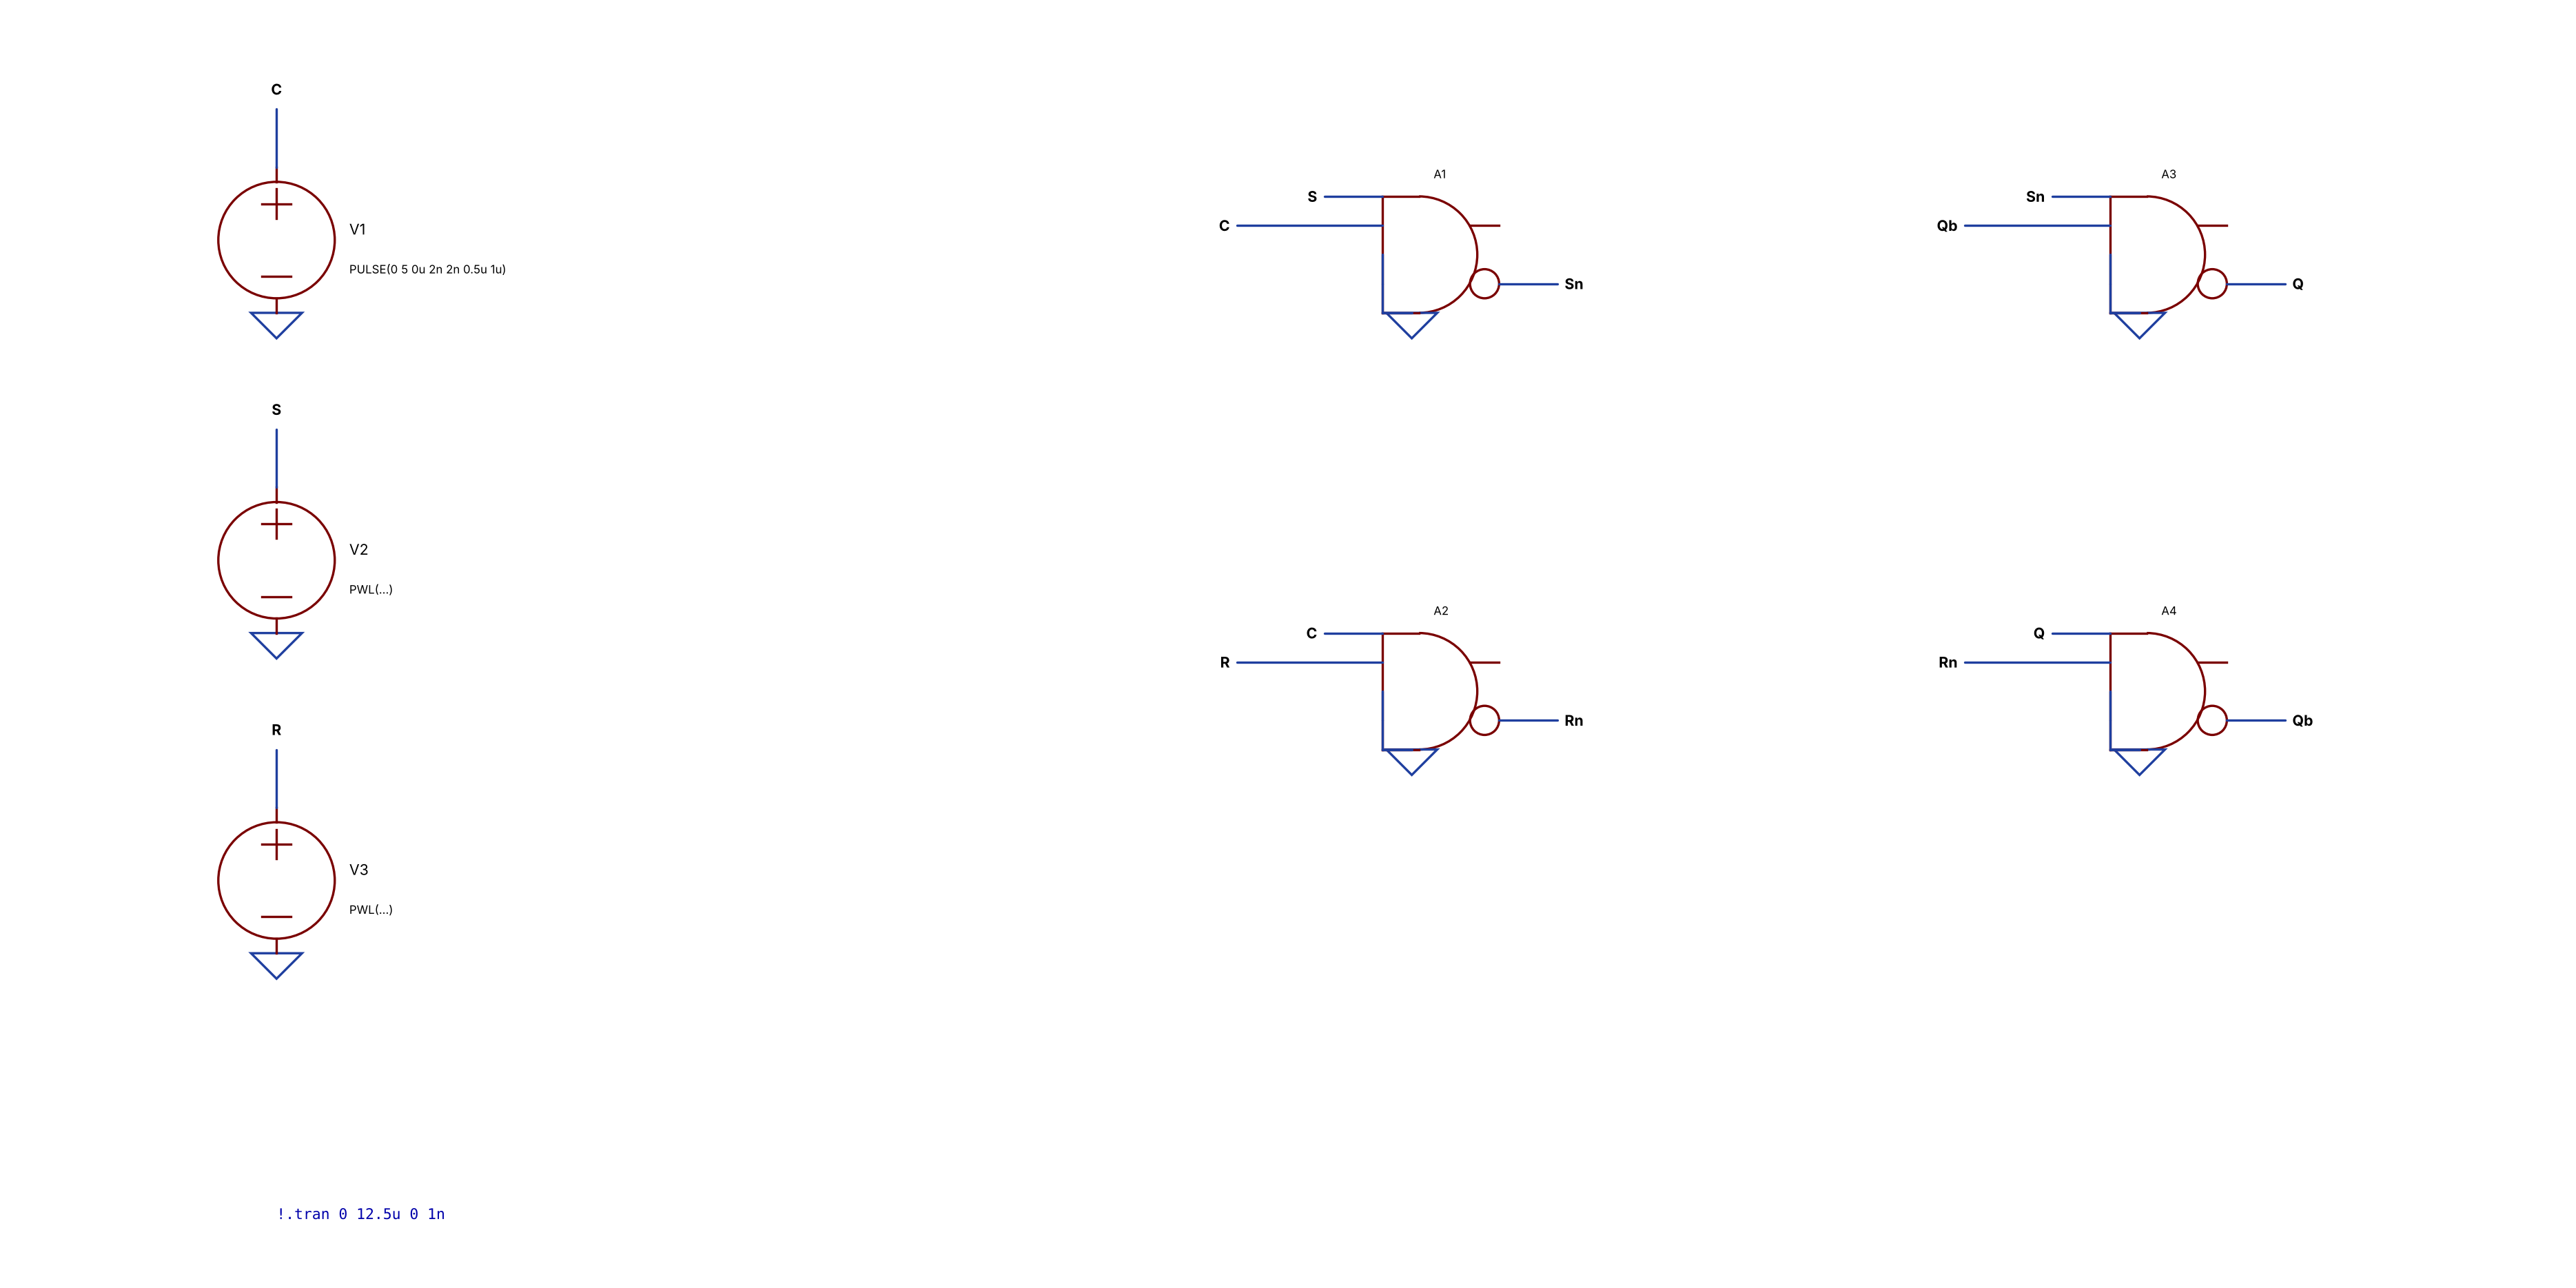
\includegraphics[width=\textwidth]{rs_sync_nand_sch.png}
\caption{Схема синхронного RS-триггера на элементах И-НЕ в LTspice (файл
\texttt{rs\_sync\_nand.asc})}
\label{fig:rs_sch}
\end{figure}

\subsection{Входные сигналы}
$C$: \texttt{PULSE(0 5 0 2n 2n 0.5u 1u)} -- $C=1$ на интервалах $[k;\,k+0{,}5]$~мкс.
Сигналы $S$ и $R$ заданы источниками \texttt{PWL} и меняются при $C=0$ (в моменты
$k+0{,}75$~мкс), чтобы в каждом такте проверялась одна комбинация: сброс, хранение,
установка, хранение, сброс, хранение, запрещённая комбинация $S=R=1$ и снова установка.
Дополнительно на интервале 8,6--8,9~мкс при $C=0$ подан импульс $S=1$ для проверки
блокировки входов. Директива: \texttt{.tran 0 12.5u 0 1n}.

\subsection{Результаты моделирования}
\begin{figure}[H]
\centering
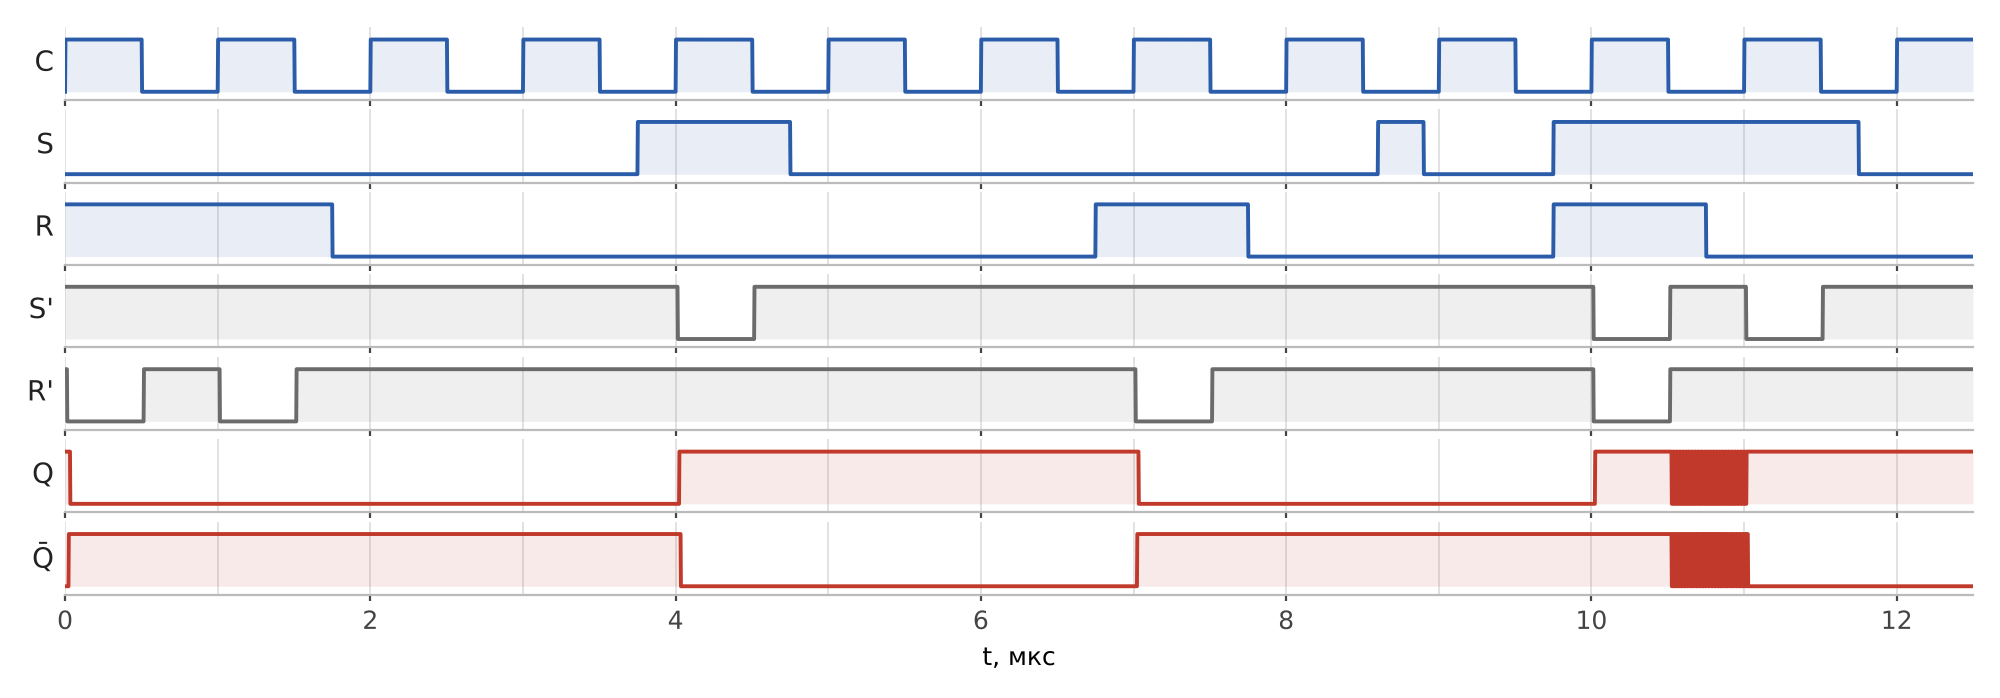
\includegraphics[width=\textwidth]{rs_sync_nand_wave.png}
\caption{Временные диаграммы синхронного RS-триггера}
\label{fig:rs_wave}
\end{figure}

\begin{table}[H]
\caption{Таблица состояний синхронного RS-триггера по результатам моделирования
(значения $Q_{n+1}$ считаны в конце такта $C=1$)}
\label{tab:rs}
\centering\small
\begin{tabular}{ccccccl}
\toprule
Такт ($C=1$), мкс & $S$ & $R$ & $Q_n$ & $Q_{n+1}$ & $\overline{Q}_{n+1}$ & Режим \\
\midrule
0--0{,}5 & 0 & 1 & -- & 0 & 1 & сброс \\
1--1{,}5 & 0 & 1 & 0 & 0 & 1 & сброс \\
2--2{,}5 & 0 & 0 & 0 & 0 & 1 & хранение \\
3--3{,}5 & 0 & 0 & 0 & 0 & 1 & хранение \\
4--4{,}5 & 1 & 0 & 0 & 1 & 0 & установка \\
5--5{,}5 & 0 & 0 & 1 & 1 & 0 & хранение \\
6--6{,}5 & 0 & 0 & 1 & 1 & 0 & хранение \\
7--7{,}5 & 0 & 1 & 1 & 0 & 1 & сброс \\
8--8{,}5 & 0 & 0 & 0 & 0 & 1 & хранение \\
9--9{,}5 & 0 & 0 & 0 & 0 & 1 & хранение \\
10--10{,}5 & 1 & 1 & 0 & 1 & 1 & запрещённая \\
11--11{,}5 & 1 & 0 & $X$ & 1 & 0 & установка \\
\midrule
8{,}6--8{,}9 ($C=0$) & 1 & 0 & 0 & 0 & 1 & вход заблокирован \\
\bottomrule
\end{tabular}
\end{table}

Полученная таблица совпадает с теоретической таблицей состояний (табл.~3 методических
указаний): при $C=0$ состояние не меняется независимо от $S$ и $R$, при $C=1$ выполняются
режимы хранения, установки и сброса.

\subsection{Анализ переходных процессов}
\textbf{Задержка.} При установке ($t=4$~мкс) сигнал проходит через два элемента: сначала
$S'$ падает через $t_d$, затем $Q$ поднимается ещё через $t_d$, и только после этого
$\nm{Q}$ падает (третий уровень). Полное время переключения триггера -- около $3t_d=30$~нс,
при этом $Q$ и $\nm{Q}$ переключаются неодновременно (рис.~\ref{fig:rs_set}).

\begin{figure}[H]
\centering
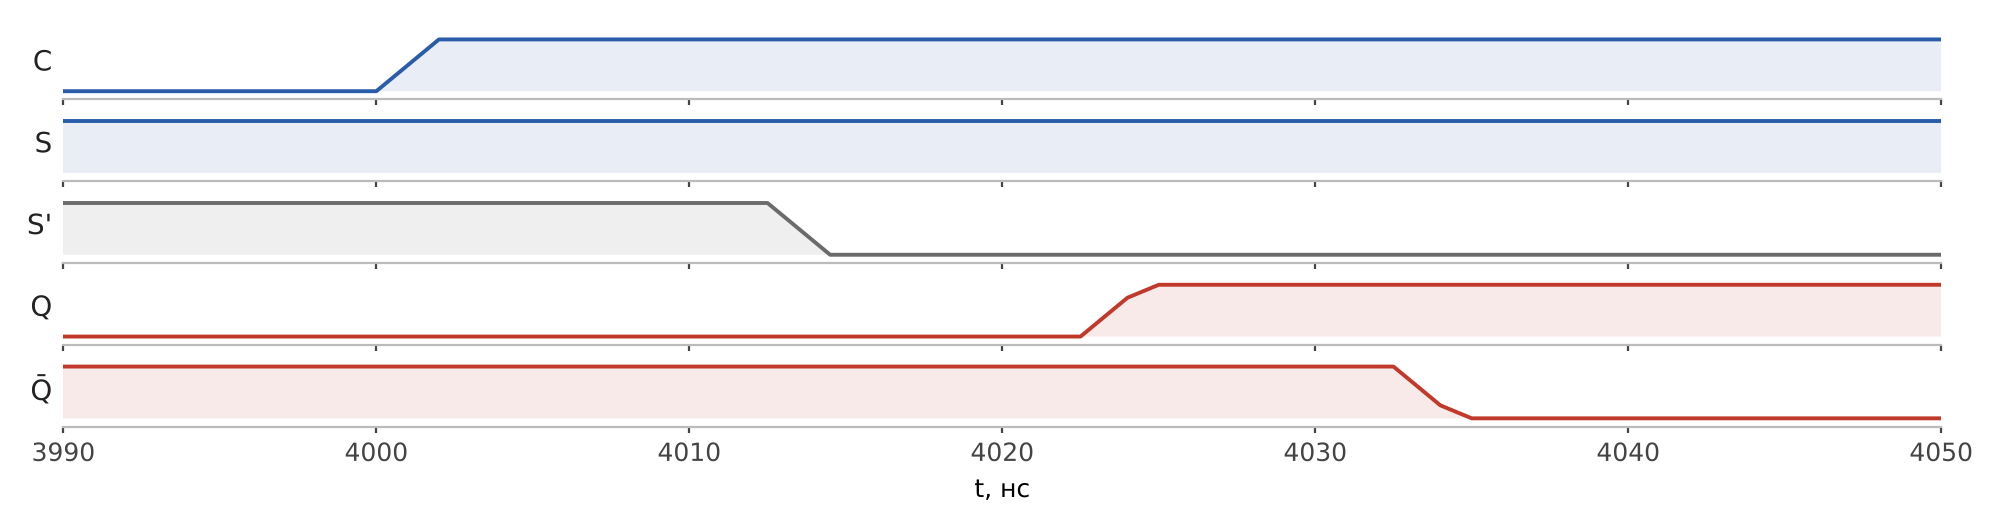
\includegraphics[width=0.9\textwidth]{rs_sync_nand_set_zoom.png}
\caption{Переходный процесс при установке триггера ($t=4$~мкс)}
\label{fig:rs_set}
\end{figure}

\textbf{Запрещённая комбинация.} При $S=R=1$ и $C=1$ (10--10,5~мкс) оба выхода равны 1,
т.\,е. $Q=\nm{Q}$ -- нарушается сама логика триггера. Ещё опаснее момент окончания такта:
$S'$ и $R'$ одновременно переходят в 1, и обе половины защёлки начинают переключаться
одновременно. В модели с одинаковыми задержками это приводит к генерации -- выходы
колеблются синфазно с периодом $2t_d=20$~нс до прихода следующего такта
(рис.~\ref{fig:rs_osc}; на рис.~\ref{fig:rs_wave} -- закрашенная область 10,5--11~мкс).
В реальной схеме из-за неравенства задержек триггер попадает в метастабильное состояние и
переходит в случайное устойчивое состояние, поэтому $Q_n$ в следующем такте обозначено $X$.
Именно поэтому комбинация $S=R=1$ называется запрещённой. Подача в 11~мкс команды
установки ($S=1, R=0$) возвращает триггер в определённое состояние $Q=1$.

\begin{figure}[H]
\centering
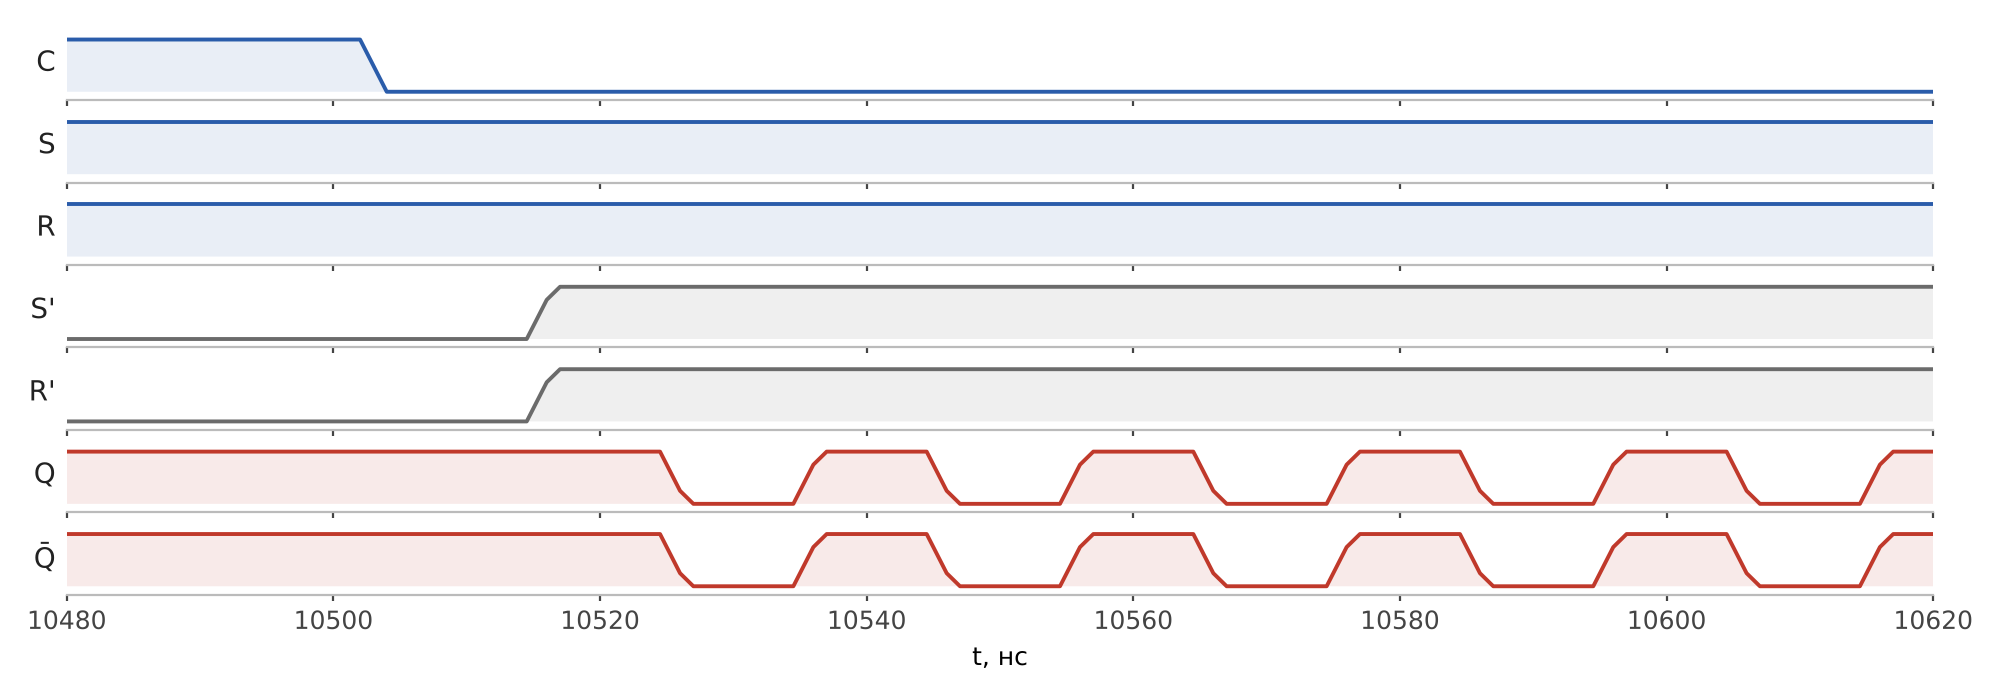
\includegraphics[width=0.9\textwidth]{rs_sync_nand_zoom.png}
\caption{Генерация после снятия запрещённой комбинации $S=R=1$ ($C$: $1\to0$ в 10,5~мкс)}
\label{fig:rs_osc}
\end{figure}

% =====================================================================
\section{Сдвигающий влево регистр}
\subsection{Принцип работы и схема}
Четырёхразрядный регистр с последовательным входом $D_{in}$ построен на четырёх D-триггерах
с общим тактовым сигналом CLK и общим сбросом CLR. Вход младшего разряда подключён к
$D_{in}$, вход каждого следующего разряда -- к выходу предыдущего:
\begin{equation}
Q_0^{n+1}=D_{in},\quad Q_1^{n+1}=Q_0^{n},\quad Q_2^{n+1}=Q_1^{n},\quad Q_3^{n+1}=Q_2^{n}.
\end{equation}
Если записывать слово как $Q_3Q_2Q_1Q_0$ (старший разряд слева), каждое слово по фронту
CLK сдвигается на один разряд влево, а новый бит вдвигается справа. Последовательный выход
-- $Q_3$, параллельный -- $Q_3\ldots Q_0$. На схеме (рис.~\ref{fig:sh_sch}) триггеры
расположены в порядке $Q_3,Q_2,Q_1,Q_0$ слева направо, так что данные перемещаются влево.

\begin{figure}[H]
\centering
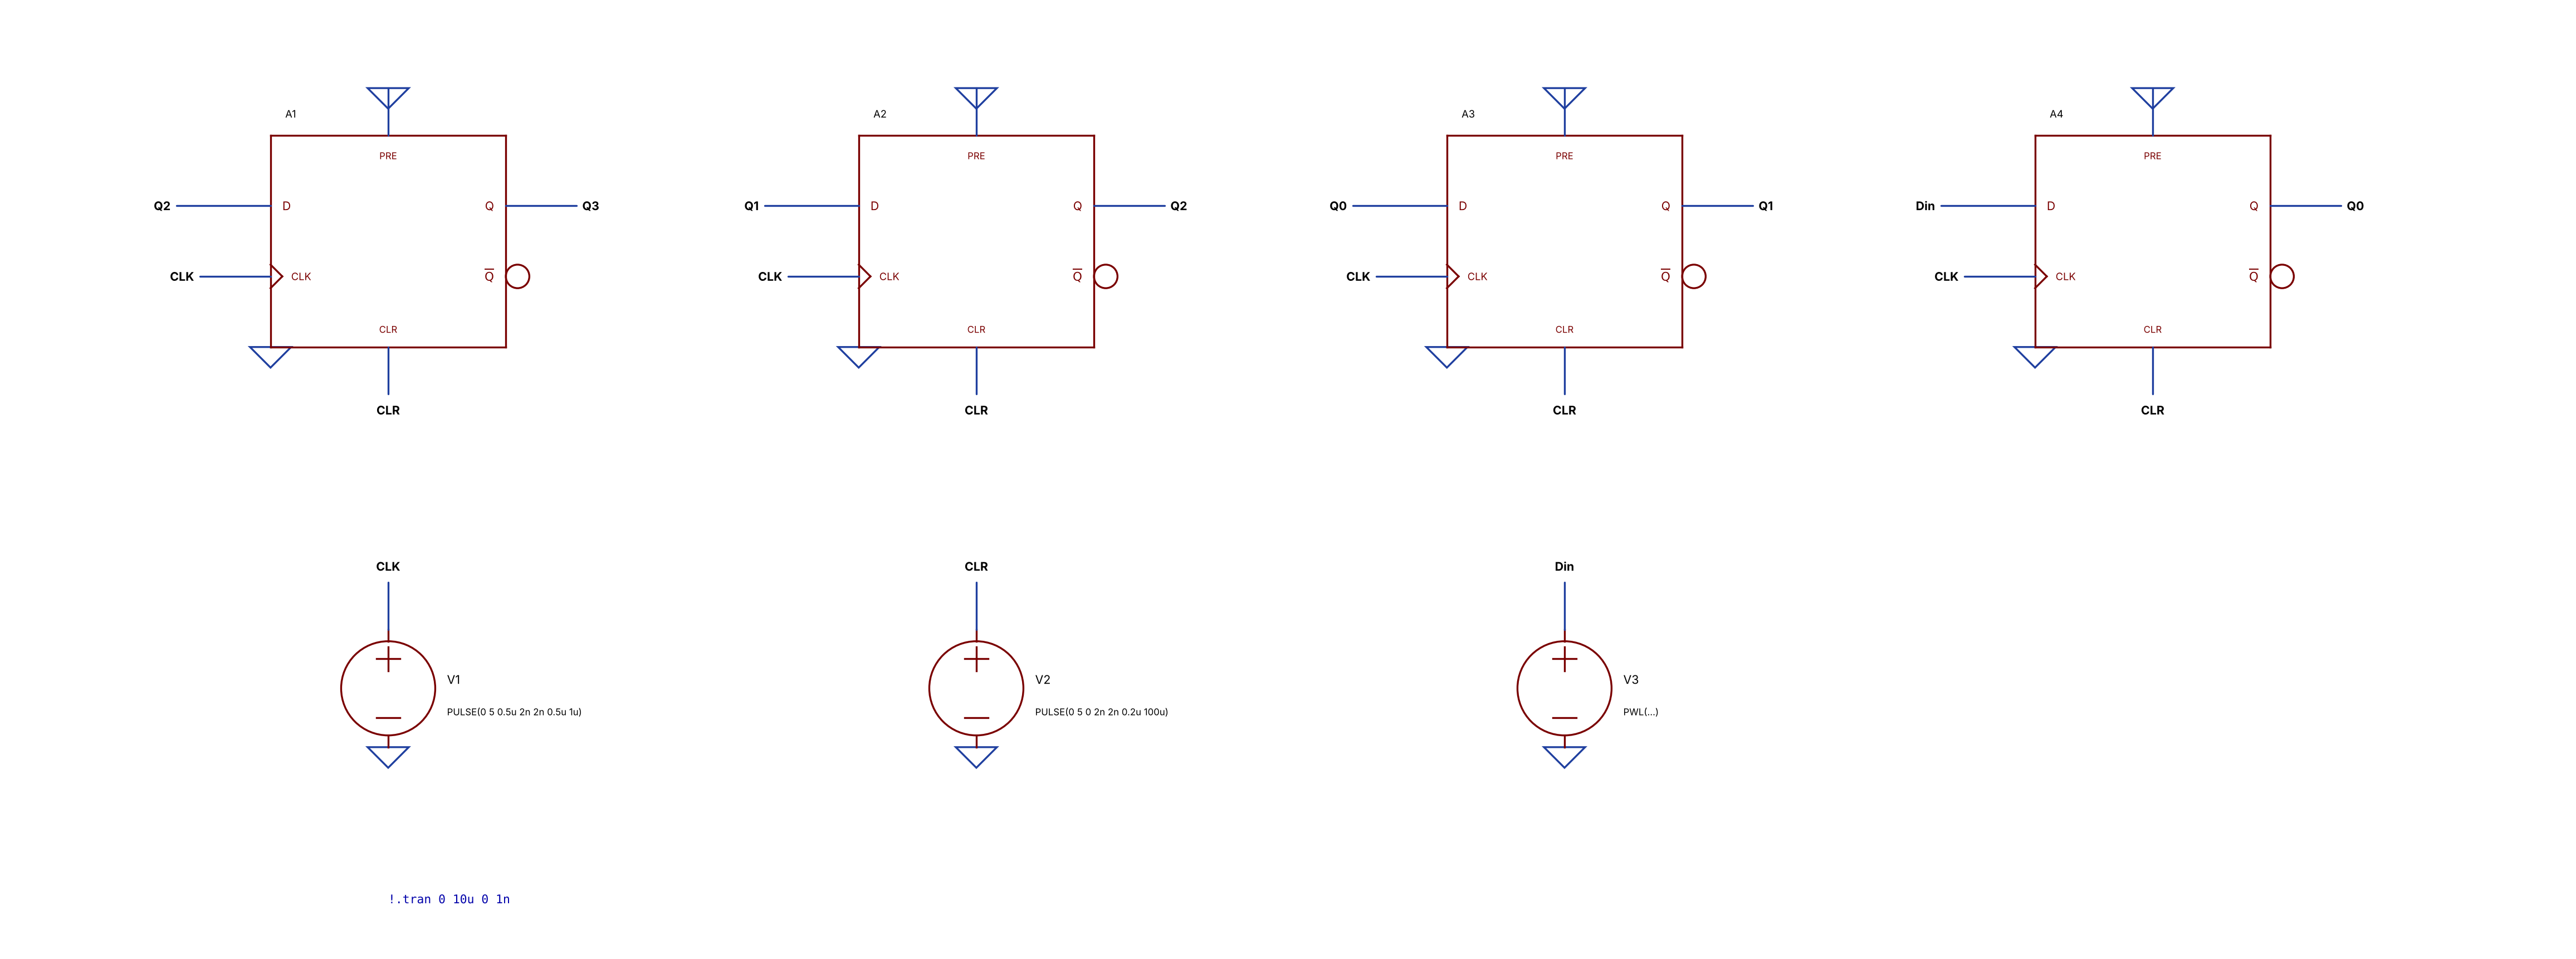
\includegraphics[width=\textwidth]{shift_left_register_sch.png}
\caption{Схема сдвигающего влево регистра в LTspice (файл
\texttt{shift\_left\_register.asc})}
\label{fig:sh_sch}
\end{figure}

\subsection{Входные сигналы}
CLK: \texttt{PULSE(0 5 0.5u 2n 2n 0.5u 1u)} (передние фронты в моменты $k+0{,}5$~мкс);
CLR: \texttt{PULSE(0 5 0 2n 2n 0.2u 100u)} -- начальный сброс; $D_{in}$: источник
\texttt{PWL}, последовательность бит 1, 1, 0, 1, 0, 0, \ldots{} (по 1~мкс на бит, смена
данных в середине паузы тактового сигнала). Директива: \texttt{.tran 0 10u 0 1n}.

\subsection{Результаты моделирования}
\begin{figure}[H]
\centering
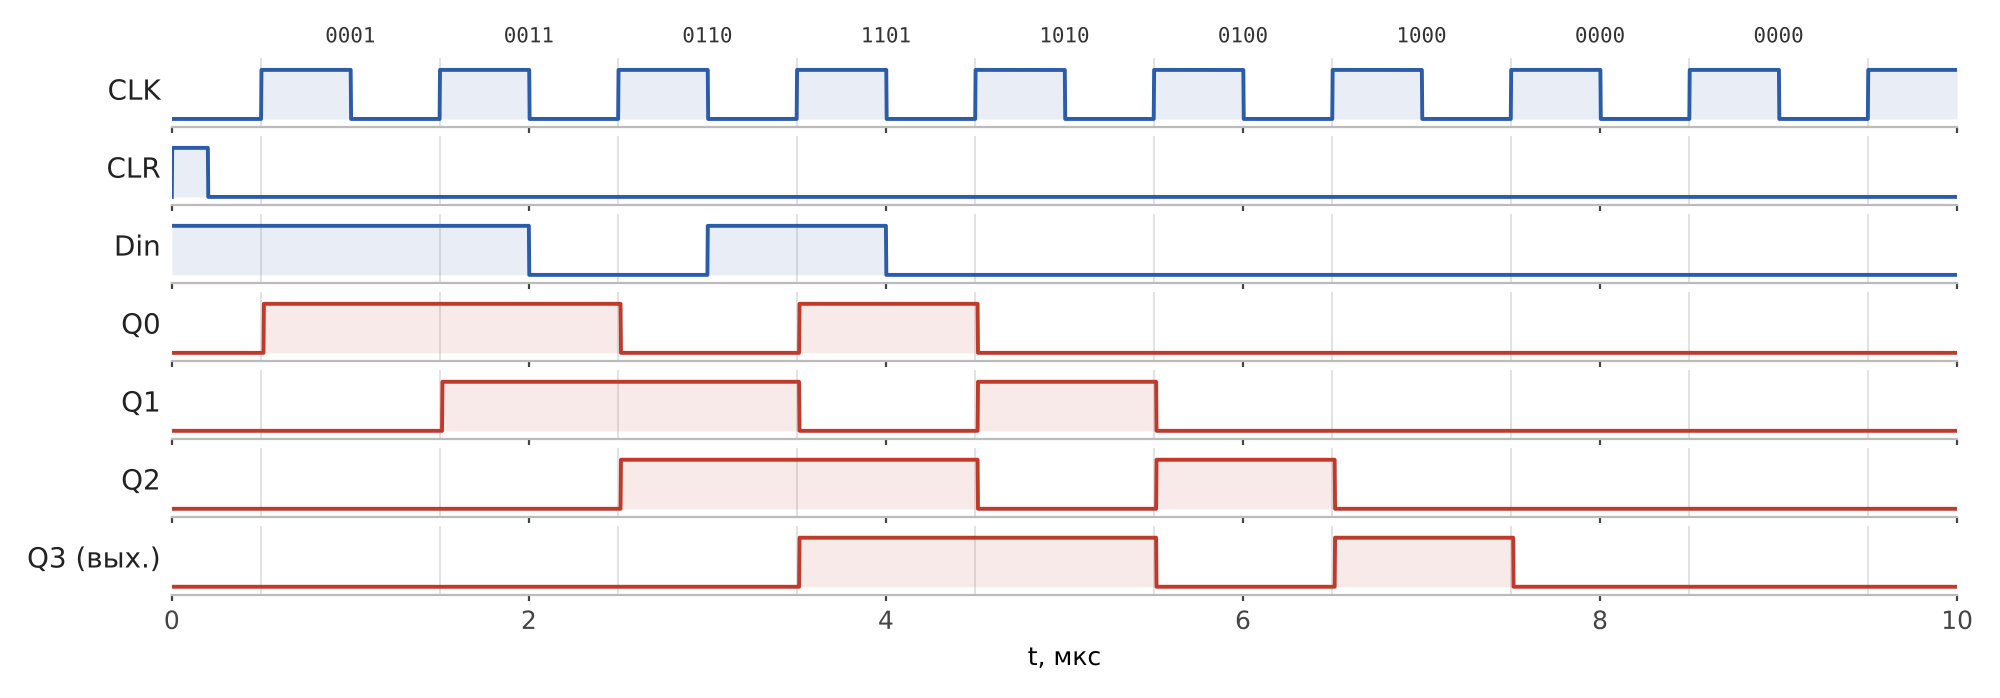
\includegraphics[width=\textwidth]{shift_left_register_wave.png}
\caption{Временные диаграммы сдвигающего влево регистра (сверху -- содержимое
$Q_3Q_2Q_1Q_0$ после фронта)}
\label{fig:sh_wave}
\end{figure}

\begin{table}[H]
\caption{Таблица состояний регистра по результатам моделирования}
\label{tab:sh}
\centering
\begin{tabular}{cc|cccc|c}
\toprule
Фронт CLK & $D_{in}$ & $Q_3$ & $Q_2$ & $Q_1$ & $Q_0$ & Слово $Q_3Q_2Q_1Q_0$ \\
\midrule
0 (после CLR) & -- & 0 & 0 & 0 & 0 & \texttt{0000} \\
1 & 1 & 0 & 0 & 0 & 1 & \texttt{0001} \\
2 & 1 & 0 & 0 & 1 & 1 & \texttt{0011} \\
3 & 0 & 0 & 1 & 1 & 0 & \texttt{0110} \\
4 & 1 & 1 & 1 & 0 & 1 & \texttt{1101} \\
5 & 0 & 1 & 0 & 1 & 0 & \texttt{1010} \\
6 & 0 & 0 & 1 & 0 & 0 & \texttt{0100} \\
7 & 0 & 1 & 0 & 0 & 0 & \texttt{1000} \\
8 & 0 & 0 & 0 & 0 & 0 & \texttt{0000} \\
9 & 0 & 0 & 0 & 0 & 0 & \texttt{0000} \\
\bottomrule
\end{tabular}
\end{table}

После четырёх тактов в регистр записано слово \texttt{1101} (первый поступивший бит
находится в старшем разряде $Q_3$), далее при $D_{in}=0$ слово продолжает сдвигаться
влево и выдвигается через $Q_3$ в последовательности 1, 1, 0, 1, после чего регистр
очищается. Результат соответствует ожидаемому.

\subsection{Анализ}
Все триггеры тактируются одним фронтом и переключаются одновременно, с задержкой
$t_d$ относительно фронта CLK. Правильная работа сдвига обеспечивается тем, что каждый
триггер защёлкивает \emph{старое} значение выхода соседа: новое значение появляется
только через $t_d$ после фронта, когда запись уже завершена. Это условие выполняется, пока
задержка триггера больше его времени удержания; при перекосе тактового сигнала (clock skew),
превышающем задержку, данные могли бы «проскочить» через два разряда за один такт.
Сигналы $D_{in}$ меняются вдали от фронтов, поэтому нарушений времени установки нет.

% =====================================================================
\section{Синхронный нисходящий счётчик}
\subsection{Принцип работы и схема}
Четырёхразрядный вычитающий счётчик построен на D-триггерах, тактируемых общим
сигналом CLK, т.\,е. все разряды переключаются одновременно. В вычитающем счётчике разряд
$Q_i$ меняет состояние, когда все младшие разряды равны нулю (происходит заём):
\begin{equation}
T_0=1,\quad T_1=\nm{Q_0},\quad T_2=\nm{Q_0}\,\nm{Q_1},\quad T_3=\nm{Q_0}\,\nm{Q_1}\,\nm{Q_2}.
\end{equation}
Т-триггер реализован как D-триггер со входом $D_i = Q_i\oplus T_i$:
\begin{equation}
D_0=\nm{Q_0},\quad D_1=Q_1\oplus\nm{Q_0},\quad D_2=Q_2\oplus T_2,\quad D_3=Q_3\oplus T_3.
\end{equation}
Логика переноса состоит из двух элементов И ($T_2$, $T_3$) и трёх элементов XOR
(рис.~\ref{fig:cnt_sch}).

\begin{figure}[H]
\centering
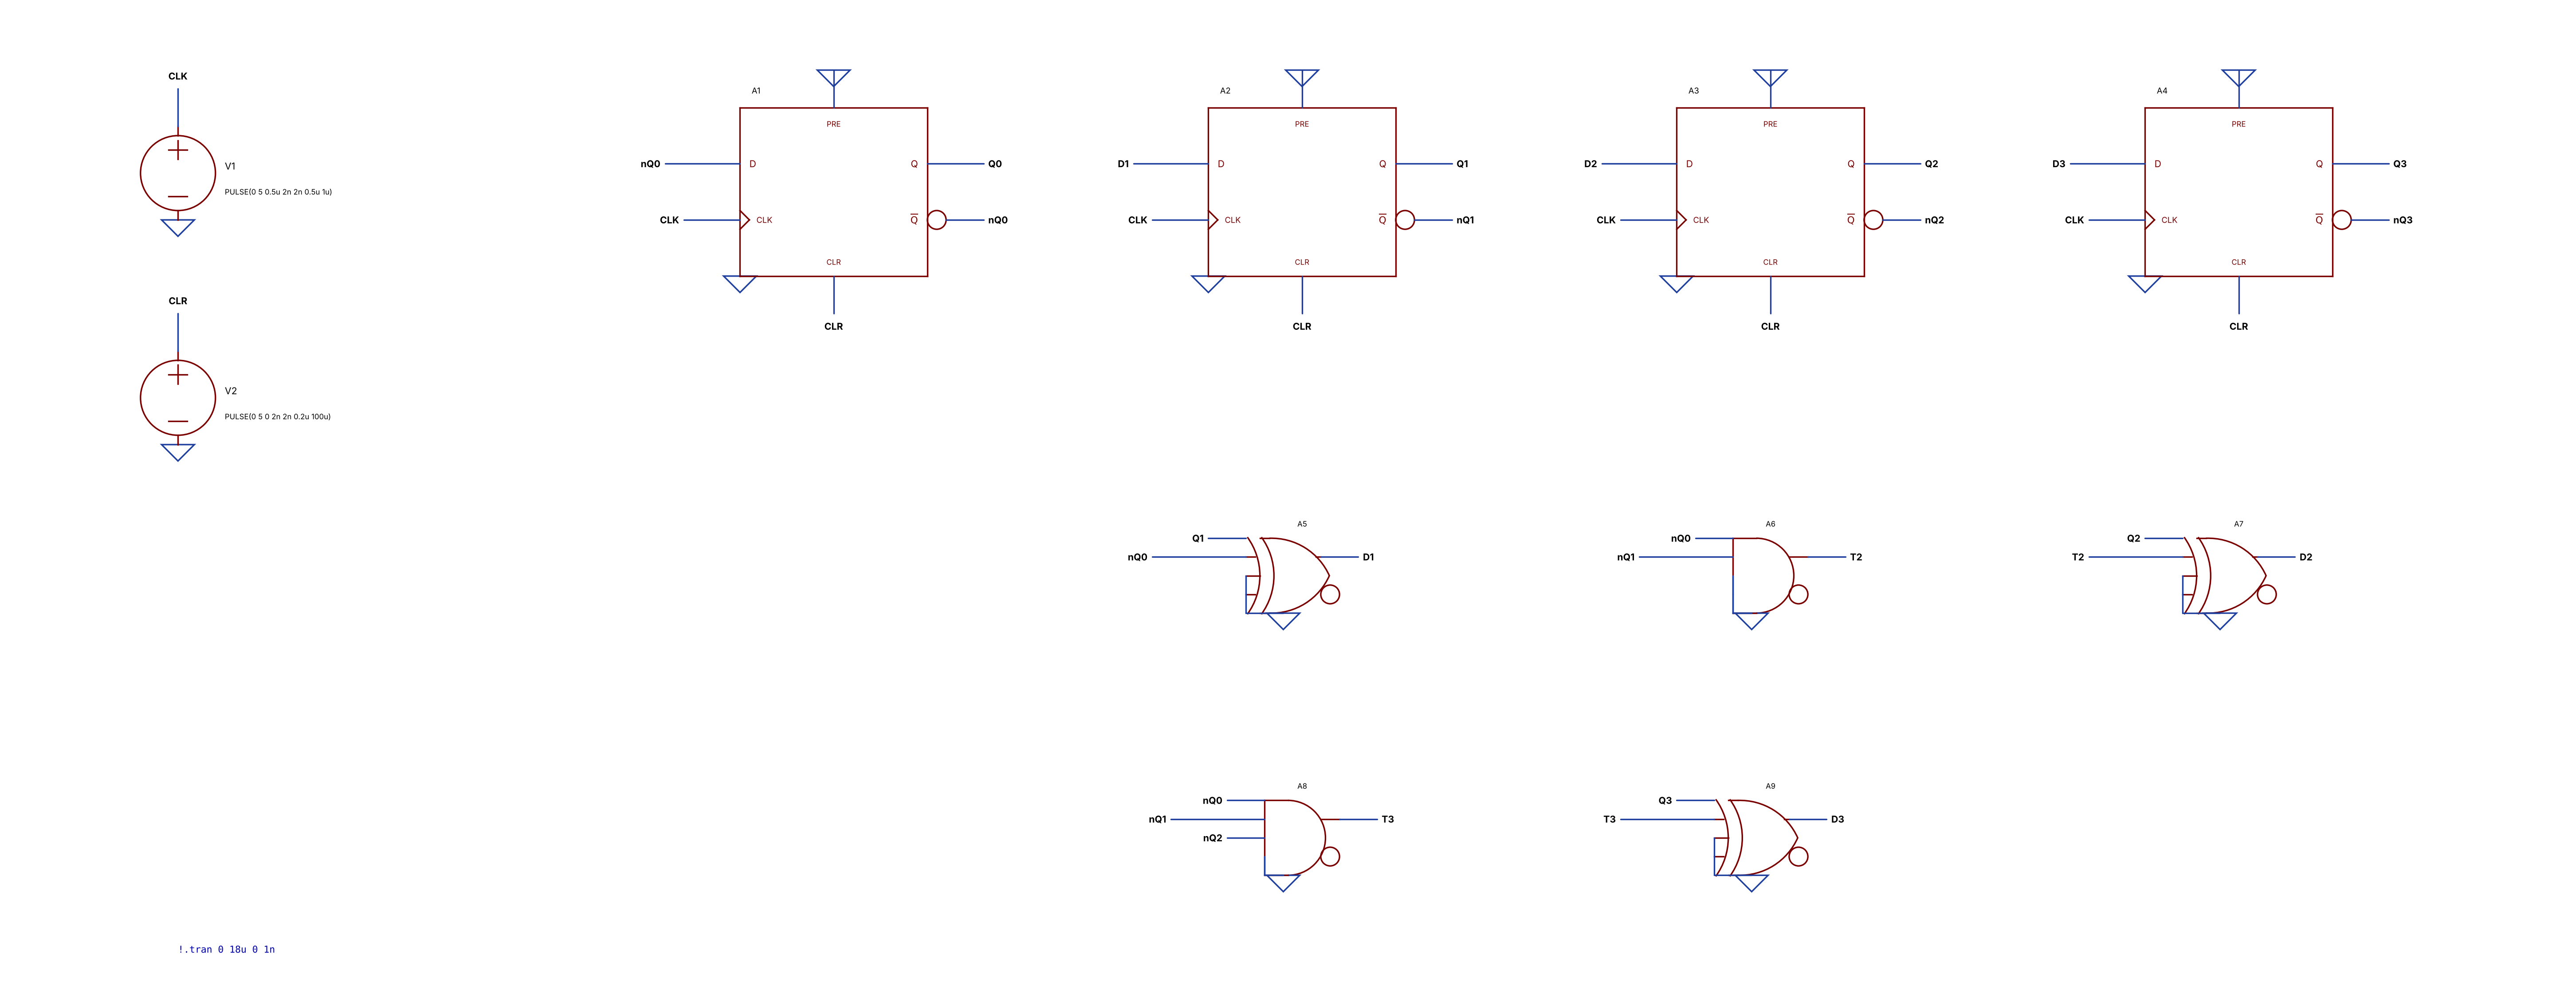
\includegraphics[width=\textwidth]{sync_down_counter_sch.png}
\caption{Схема синхронного нисходящего счётчика в LTspice (файл
\texttt{sync\_down\_counter.asc})}
\label{fig:cnt_sch}
\end{figure}

\subsection{Входные сигналы}
CLK: \texttt{PULSE(0 5 0.5u 2n 2n 0.5u 1u)}; CLR: \texttt{PULSE(0 5 0 2n 2n 0.2u 100u)}
(начальный сброс в 0000). Директива \texttt{.tran 0 18u 0 1n} -- 17 тактов, т.\,е. полный
цикл из 16 состояний и переход на следующий цикл.

\subsection{Результаты моделирования}
\begin{figure}[H]
\centering
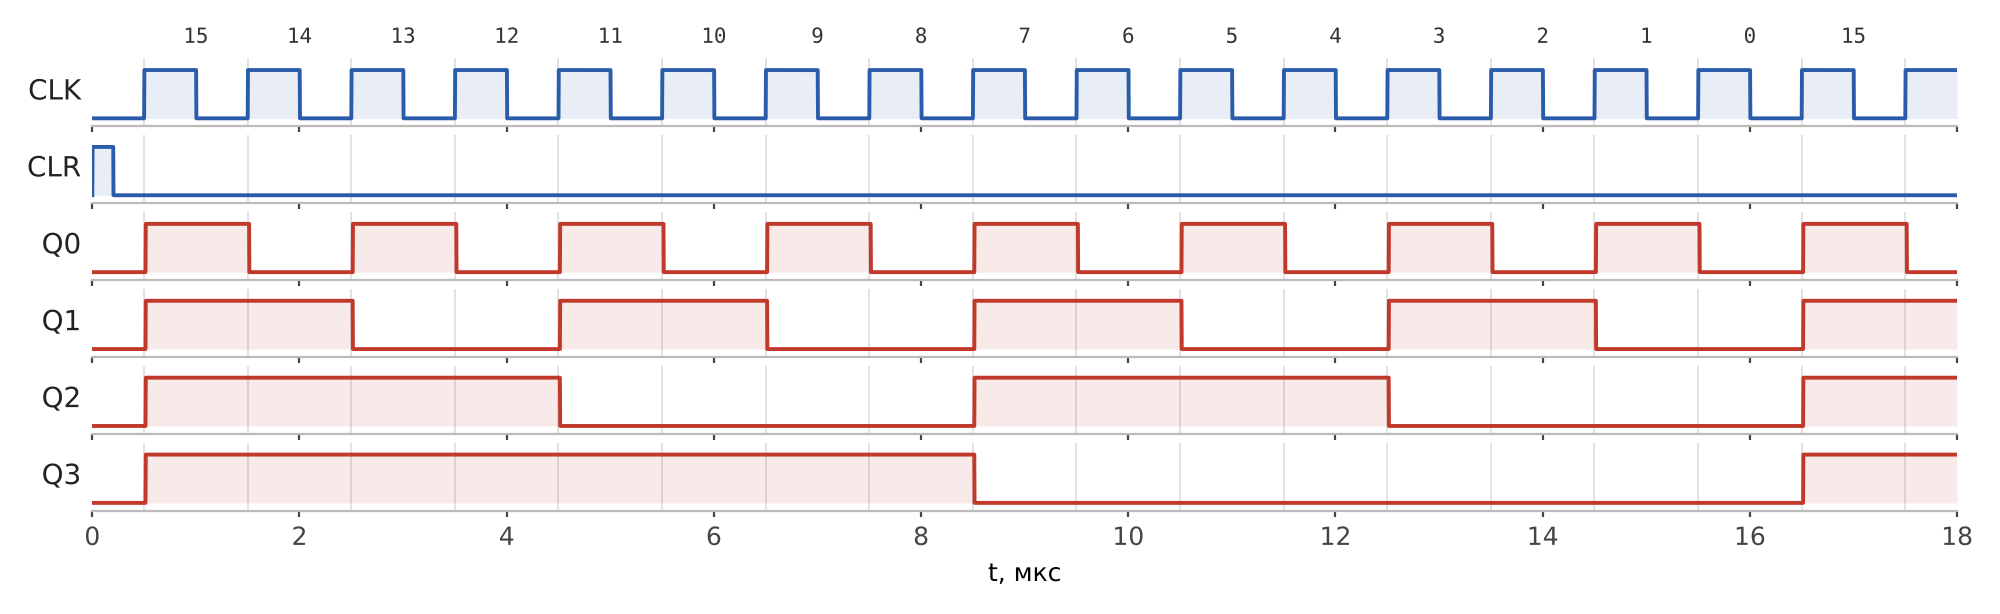
\includegraphics[width=\textwidth]{sync_down_counter_wave.png}
\caption{Временные диаграммы синхронного нисходящего счётчика (сверху -- десятичное
значение $Q_3Q_2Q_1Q_0$ после каждого фронта)}
\label{fig:cnt_wave}
\end{figure}

\begin{table}[H]
\caption{Таблица состояний счётчика по результатам моделирования}
\label{tab:cnt}
\centering\small
\begin{tabular}{c|cccc|c}
\toprule
Фронт CLK & $Q_3$ & $Q_2$ & $Q_1$ & $Q_0$ & Десятичное \\
\midrule
0 (после CLR) & 0 & 0 & 0 & 0 & 0 \\
1 & 1 & 1 & 1 & 1 & 15 \\
2 & 1 & 1 & 1 & 0 & 14 \\
3 & 1 & 1 & 0 & 1 & 13 \\
4 & 1 & 1 & 0 & 0 & 12 \\
5 & 1 & 0 & 1 & 1 & 11 \\
6 & 1 & 0 & 1 & 0 & 10 \\
7 & 1 & 0 & 0 & 1 & 9 \\
8 & 1 & 0 & 0 & 0 & 8 \\
9 & 0 & 1 & 1 & 1 & 7 \\
10 & 0 & 1 & 1 & 0 & 6 \\
11 & 0 & 1 & 0 & 1 & 5 \\
12 & 0 & 1 & 0 & 0 & 4 \\
13 & 0 & 0 & 1 & 1 & 3 \\
14 & 0 & 0 & 1 & 0 & 2 \\
15 & 0 & 0 & 0 & 1 & 1 \\
16 & 0 & 0 & 0 & 0 & 0 \\
17 & 1 & 1 & 1 & 1 & 15 \\
\bottomrule
\end{tabular}
\end{table}

После сброса счётчик находится в состоянии 0000; первый фронт CLK переводит его в
1111 (15), далее каждое срабатывание уменьшает значение на 1: $15\to14\to\ldots\to1\to0$,
после 0 следует снова 15. Модуль счёта равен 16, последовательность совпадает с
ожидаемой.

\subsection{Анализ переходных процессов}
На рис.~\ref{fig:cnt_zoom} показан фронт CLK в момент 8,5~мкс, при котором происходит
переход $1000\to0111$ -- меняются все четыре разряда. Все выходы $Q_0\ldots Q_3$
переключаются \emph{одновременно}, примерно через 14~нс после начала фронта (задержка
триггера $t_d$ плюс время нарастания тактового сигнала до порога). В асинхронном
(последовательном) счётчике разряды переключались бы друг за другом, с суммарной задержкой
$4t_d$, и на выходе кратковременно появлялись бы ложные коды; в синхронном счётчике этого нет.

Сигналы логики переноса $T_2$, $T_3$, $D_2$, $D_3$ устанавливаются позже, через 1--2
уровня элементов, и на $D_2$, $D_3$ видны кратковременные ложные импульсы (около 10~нс),
вызванные разной длиной путей. Они не влияют на работу, так как приходятся на середину
такта и заканчиваются задолго до следующего фронта. Максимальная частота тактирования
ограничивается суммой: задержка триггера + задержка логики (И и XOR, $2t_d$) + время
установки триггера, т.\,е. порядка $3t_d\approx30$~нс в данной модели.

\begin{figure}[H]
\centering
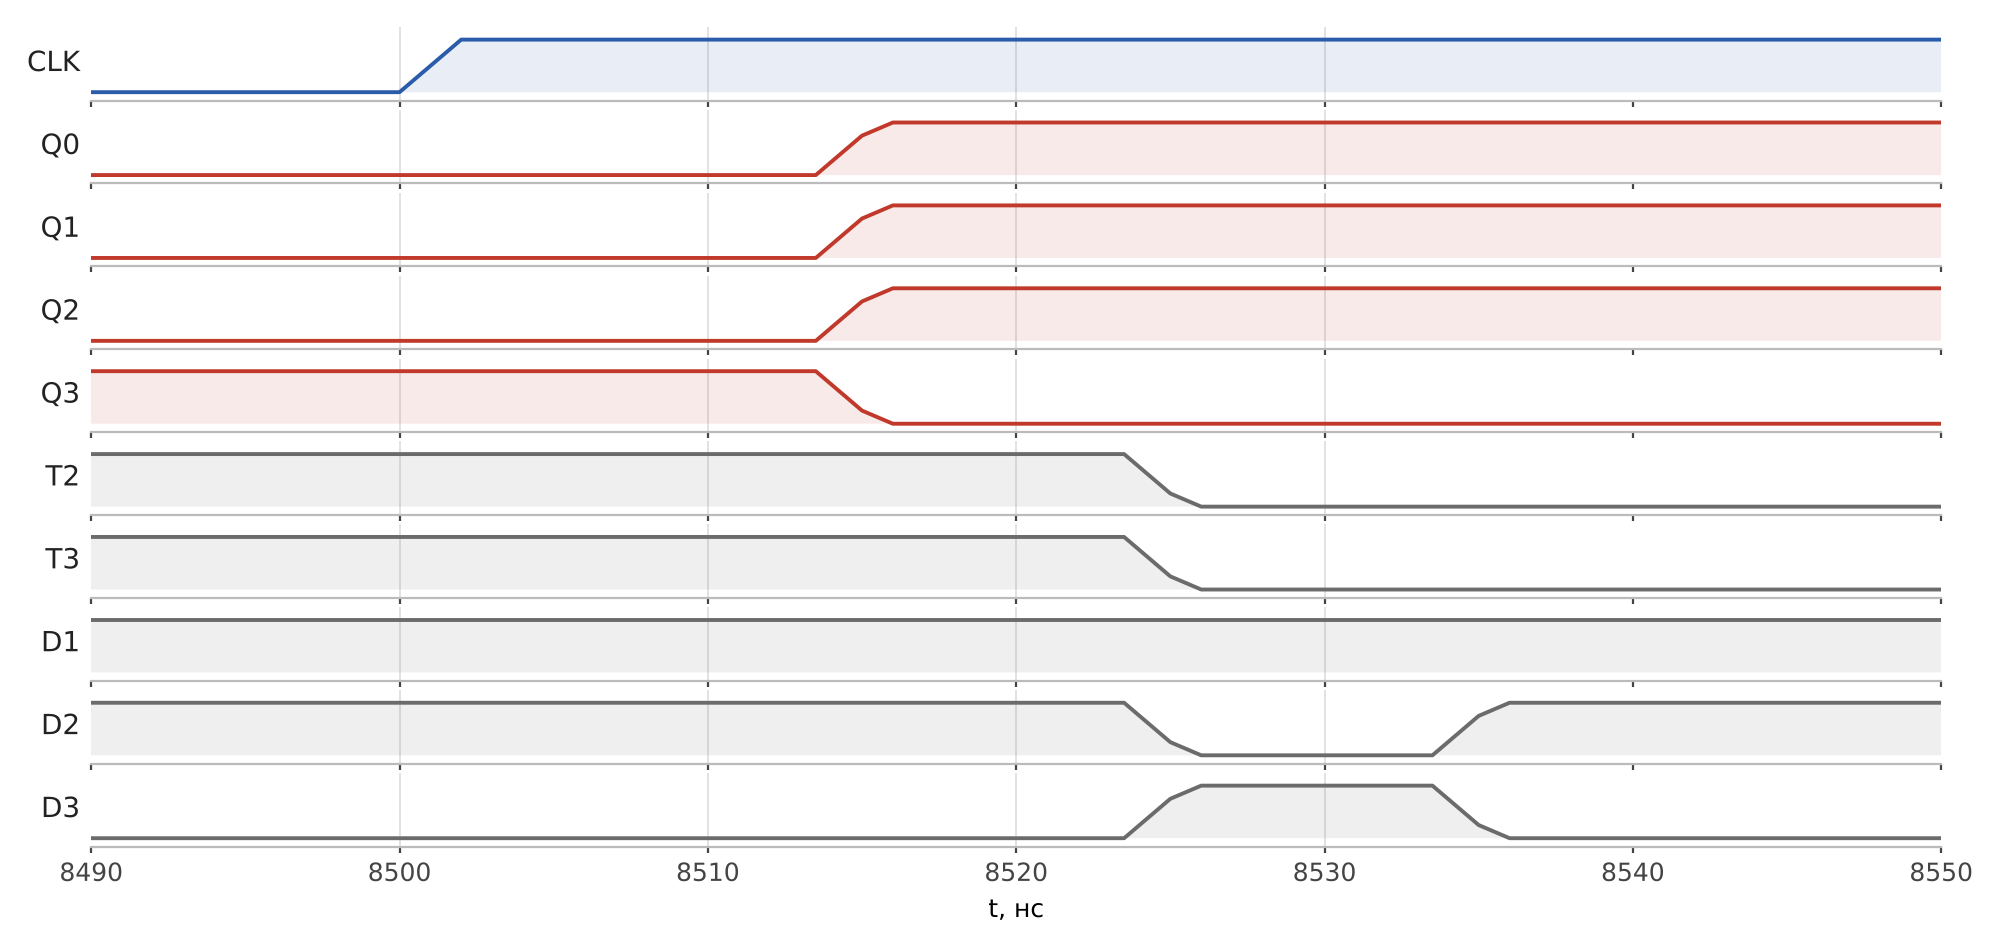
\includegraphics[width=0.9\textwidth]{sync_down_counter_zoom.png}
\caption{Переход $1000\to0111$ на фронте CLK ($t=8{,}5$~мкс): одновременное
переключение разрядов}
\label{fig:cnt_zoom}
\end{figure}

% =====================================================================
\section{Ответы на контрольные вопросы}
\textbf{1. Чем отличается D-триггер от JK?}
D-триггер имеет один информационный вход: по активному фронту (уровню) он записывает
значение $D$, $Q_{n+1}=D$, и режима хранения при наличии такта не имеет. JK-триггер имеет два
входа: $J$ -- установка, $K$ -- сброс, $J=K=0$ -- хранение, а комбинация $J=K=1$ не
запрещена, как у RS-триггера, а вызывает переключение (счётный режим):
$Q_{n+1}=J\,\nm{Q_n}+\nm{K}\,Q_n$.

\textbf{2. Как реализуется синхронный счётчик?}
Все триггеры тактируются одним общим сигналом, а необходимость переключения каждого разряда
определяет комбинационная логика: для суммирующего счётчика $T_i=Q_0Q_1\ldots Q_{i-1}$,
для вычитающего $T_i=\nm{Q_0}\,\nm{Q_1}\ldots\nm{Q_{i-1}}$. Т-функция реализуется
Т- или JK-триггерами ($J=K=T_i$) либо D-триггерами с $D_i=Q_i\oplus T_i$, как в данной работе.

\textbf{3. Что произойдёт при наложении тактов и управляющих сигналов?}
Если информационный или управляющий сигнал меняется одновременно с активным фронтом такта
(нарушены времена установки и удержания), результат записи становится неопределённым:
триггер может записать старое или новое значение или попасть в метастабильное состояние.
Асинхронные сигналы (CLR, PRE) имеют приоритет над тактовым, но их снятие вблизи фронта
также приводит к неопределённости. Поэтому управляющие сигналы меняют в паузах между
фронтами, как это сделано в моделировании.

\textbf{4. Как определить направление сдвига регистра?}
По тому, к какому соседу подключён D-вход каждого разряда. Если $D_i=Q_{i-1}$ (вход
младшего разряда -- от $D_{in}$), данные перемещаются от младших разрядов к старшим --
сдвиг влево (умножение на 2). Если $D_i=Q_{i+1}$ и последовательный вход подключён к
старшему разряду -- сдвиг вправо (деление на 2). Экспериментально направление видно по
временным диаграммам: бит появляется сначала на $Q_0$, затем на $Q_1$ и т.\,д.

\textbf{5. Какие состояния считаются запрещёнными для RS-триггера?}
Для RS-триггера на элементах ИЛИ-НЕ -- $S=R=1$, для асинхронного триггера на И-НЕ с
инверсными входами -- $\nm{S}=\nm{R}=0$, для синхронного -- $S=R=1$ при $C=1$. В этом
состоянии оба выхода принимают одинаковое значение ($Q=\nm{Q}$), а при одновременном снятии
сигналов состояние триггера непредсказуемо (гонка, генерация или метастабильность), что
и подтвердило моделирование.

% =====================================================================
\section*{Выводы}
\addcontentsline{toc}{section}{Выводы}
\begin{enumerate}[leftmargin=*, label=\arabic*.]
\item Синхронный RS-триггер на четырёх элементах И-НЕ работает в соответствии с таблицей
состояний: при $C=0$ входы заблокированы, при $C=1$ выполняются хранение, установка и
сброс. Время переключения -- около $3t_d$. Комбинация $S=R=1$ приводит к $Q=\nm{Q}=1$, а
после окончания такта -- к генерации (метастабильности), что подтверждает её запрещённость.
\item Четырёхразрядный сдвигающий влево регистр на D-триггерах правильно принимает
последовательный код (после 4 тактов записано слово 1101), сдвигает его к старшим разрядам
и выдаёт через $Q_3$.
\item Синхронный нисходящий счётчик проходит все 16 состояний $15\to0$ и возвращается в 15;
все разряды переключаются одновременно, без промежуточных ложных кодов, характерных для
асинхронных счётчиков. Кратковременные сбои логики переноса не влияют на результат, так как
затухают до следующего фронта.
\item Основное отличие от комбинационных схем -- наличие памяти: выходы зависят от
предыдущего состояния и меняются только по такту, поэтому важны временные соотношения между
тактом и входными сигналами (время установки, удержания и задержка распространения).
\end{enumerate}

\section*{Список литературы}
\addcontentsline{toc}{section}{Список литературы}
\begin{enumerate}[leftmargin=*, label=\arabic*.]
\item Хоровиц П., Хилл У. Искусство схемотехники / Пер. с англ. Изд. 2-е. -- М.: БИНОМ, 2014. -- 740 с.
\item Бойко В.\,И. Схемотехника электронных систем. Аналоговые и импульсные устройства. -- 2004.
\end{enumerate}

\end{document}
